% !TeX root = ../thuthesis-example.tex

\chapter{\emph{insertRecords} 写入请求序列化设计与实现}
第 \ref{chap:client-design} 章介绍了客户端对数据的预处理工作,在客户端的预处理结束后,写入请求需要通过 RPC 层序列化为字节流,传输到服务器侧,再反序列化为写入请求被 IoTDB 服务器处理。本章将介绍在新 \emph{insertRecords} 写入机制中,在 RPC 层序列化写入请求时的数据包结构设计与实现。

\section{写入请求序列化的设计目标}
正如 \ref{sec:chap2-sec3} 节中所介绍到的,对写入请求的序列化是一个需要权衡的过程:使用复杂的包结构设计可以让请求序列化得到的字节流很小,通过网络传输的开销比较低,但是序列化与反序列化的开销则很大;使用简单的包结构可以减少序列化与反序列化的开销,但是序列化得到的字节流较大,通过网络传输的开销较高。在设计时,设计者需要把握好压缩率与复杂度的平衡点,以获取综合最优的性能。

在对 \emph{insertRecords} 的写入请求进行序列化时,本文的设计目标如下:
\begin{enumerate}
  \item 相比于目前简单的序列化方案,新的序列化方案需要针对时序数据的特点,对数据进行一定程度的压缩,以减小数据包的体积,降低网络传输延迟;
  \item 数据序列化的资源开销需要可控,对 CPU 资源、内存资源的使用要较为轻量;
  \item 数据序列化设计需要具有可拓展性,以保证未来对序列化方案中增加内容时可以保证兼容性。
\end{enumerate}
针对以上以上的设计目标,本文设计了新的 \emph{insertRecords} 写入请求序列化方案。

\section{写入请求序列化总体设计}
\begin{figure}
  \centering
  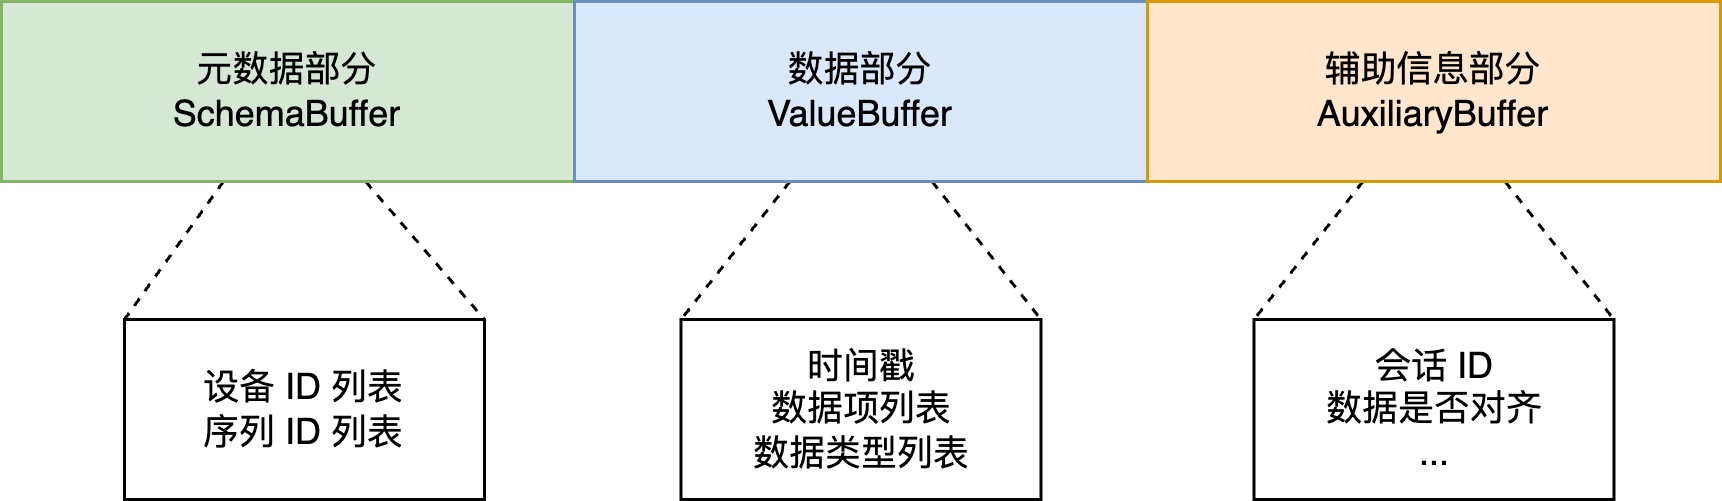
\includegraphics[width=0.9\linewidth]{rpc-general-design.png}
  \caption{写入请求序列化总体设计}
  \label{fig:rpc-general-design}
\end{figure}

在 \ref{sec:chap3-sec2-2-1} 节中,本文介绍了目前 IoTDB 在 Thrift 中对 \emph{insertRecords} 请求的定义。根据各个字段的实际含义,我们可以将它们分成三大部分:元数据部分、数据部分和辅助信息部分。

元数据部分包括设备 ID 和时间序列 ID,它们描述了待写入数据所对应的时间序列都信息。这部分的数据的呈现形式是文本形式,并且其重复度较高,这里的重复度体现在两个方面:
\begin{itemize}
  \item 同一设备或者不同设备的时间序列可能具有相同的 ID,因为它们在现实生活中对应了同样一种类型的实体,例如同样类型的传感器。
  \item 不同设备之间存在部分重复的内容。这是因为 IoTDB 的设备 ID 遵循一种树形的结构,形如 "root.层级1.层级2.层级3"。如果两个设备位于层级树的同一个子树中,那么它们的 ID 中会包含许多相同的部分。
\end{itemize}
针对以上的两个特征,元数据部分非常适合使用字典编码(Dictionary Encoding)进行处理。在本工作的实现中,将元数据部分编码后得到的结果单独保存为一个字节流。

数据部分主要包含时间戳、数值项与数值项的类型。时间戳全都为 8 字节的长整形数据,并且同一个写入请求中不同记录的时间戳可能非常接近;数值项数据可能包含各个类型的数据,如浮点数、整数、字符串等;数据项则都为 1 字节的枚举类型(Enumeration)。数据部分是写入请求序列化后体积最大的部分,对这部分数据进行较为精细化的压缩可以有效减小整个写入请求序列化后的体积。这一部分序列化后的结果也会单独保存为一个字节流。

辅助信息部分主要包括一些标志信息,辅助写入过程中的非核心流程,这部分数据包含会话 ID、数据是否按时间对齐的标志等。这部分数据可能由若干个不同数据类型的标志组成,序列化后的总体积不会很大,因此不需要进行压缩。在未来,\emph{insertRecords} 写入请求中可能会添加更多的辅助信息,因此辅助信息的序列化需要保持一定的拓展性。这一部分序列化后的结果也会单独保存为一个字节流。

下面,本文将分别介绍元数据部分、数据部分和辅助信息部分的序列化设计方案。



\section{写入请求元数据部分序列化与反序列化方案设计}
\subsection{序列化过程}
\begin{figure}
  \centering
  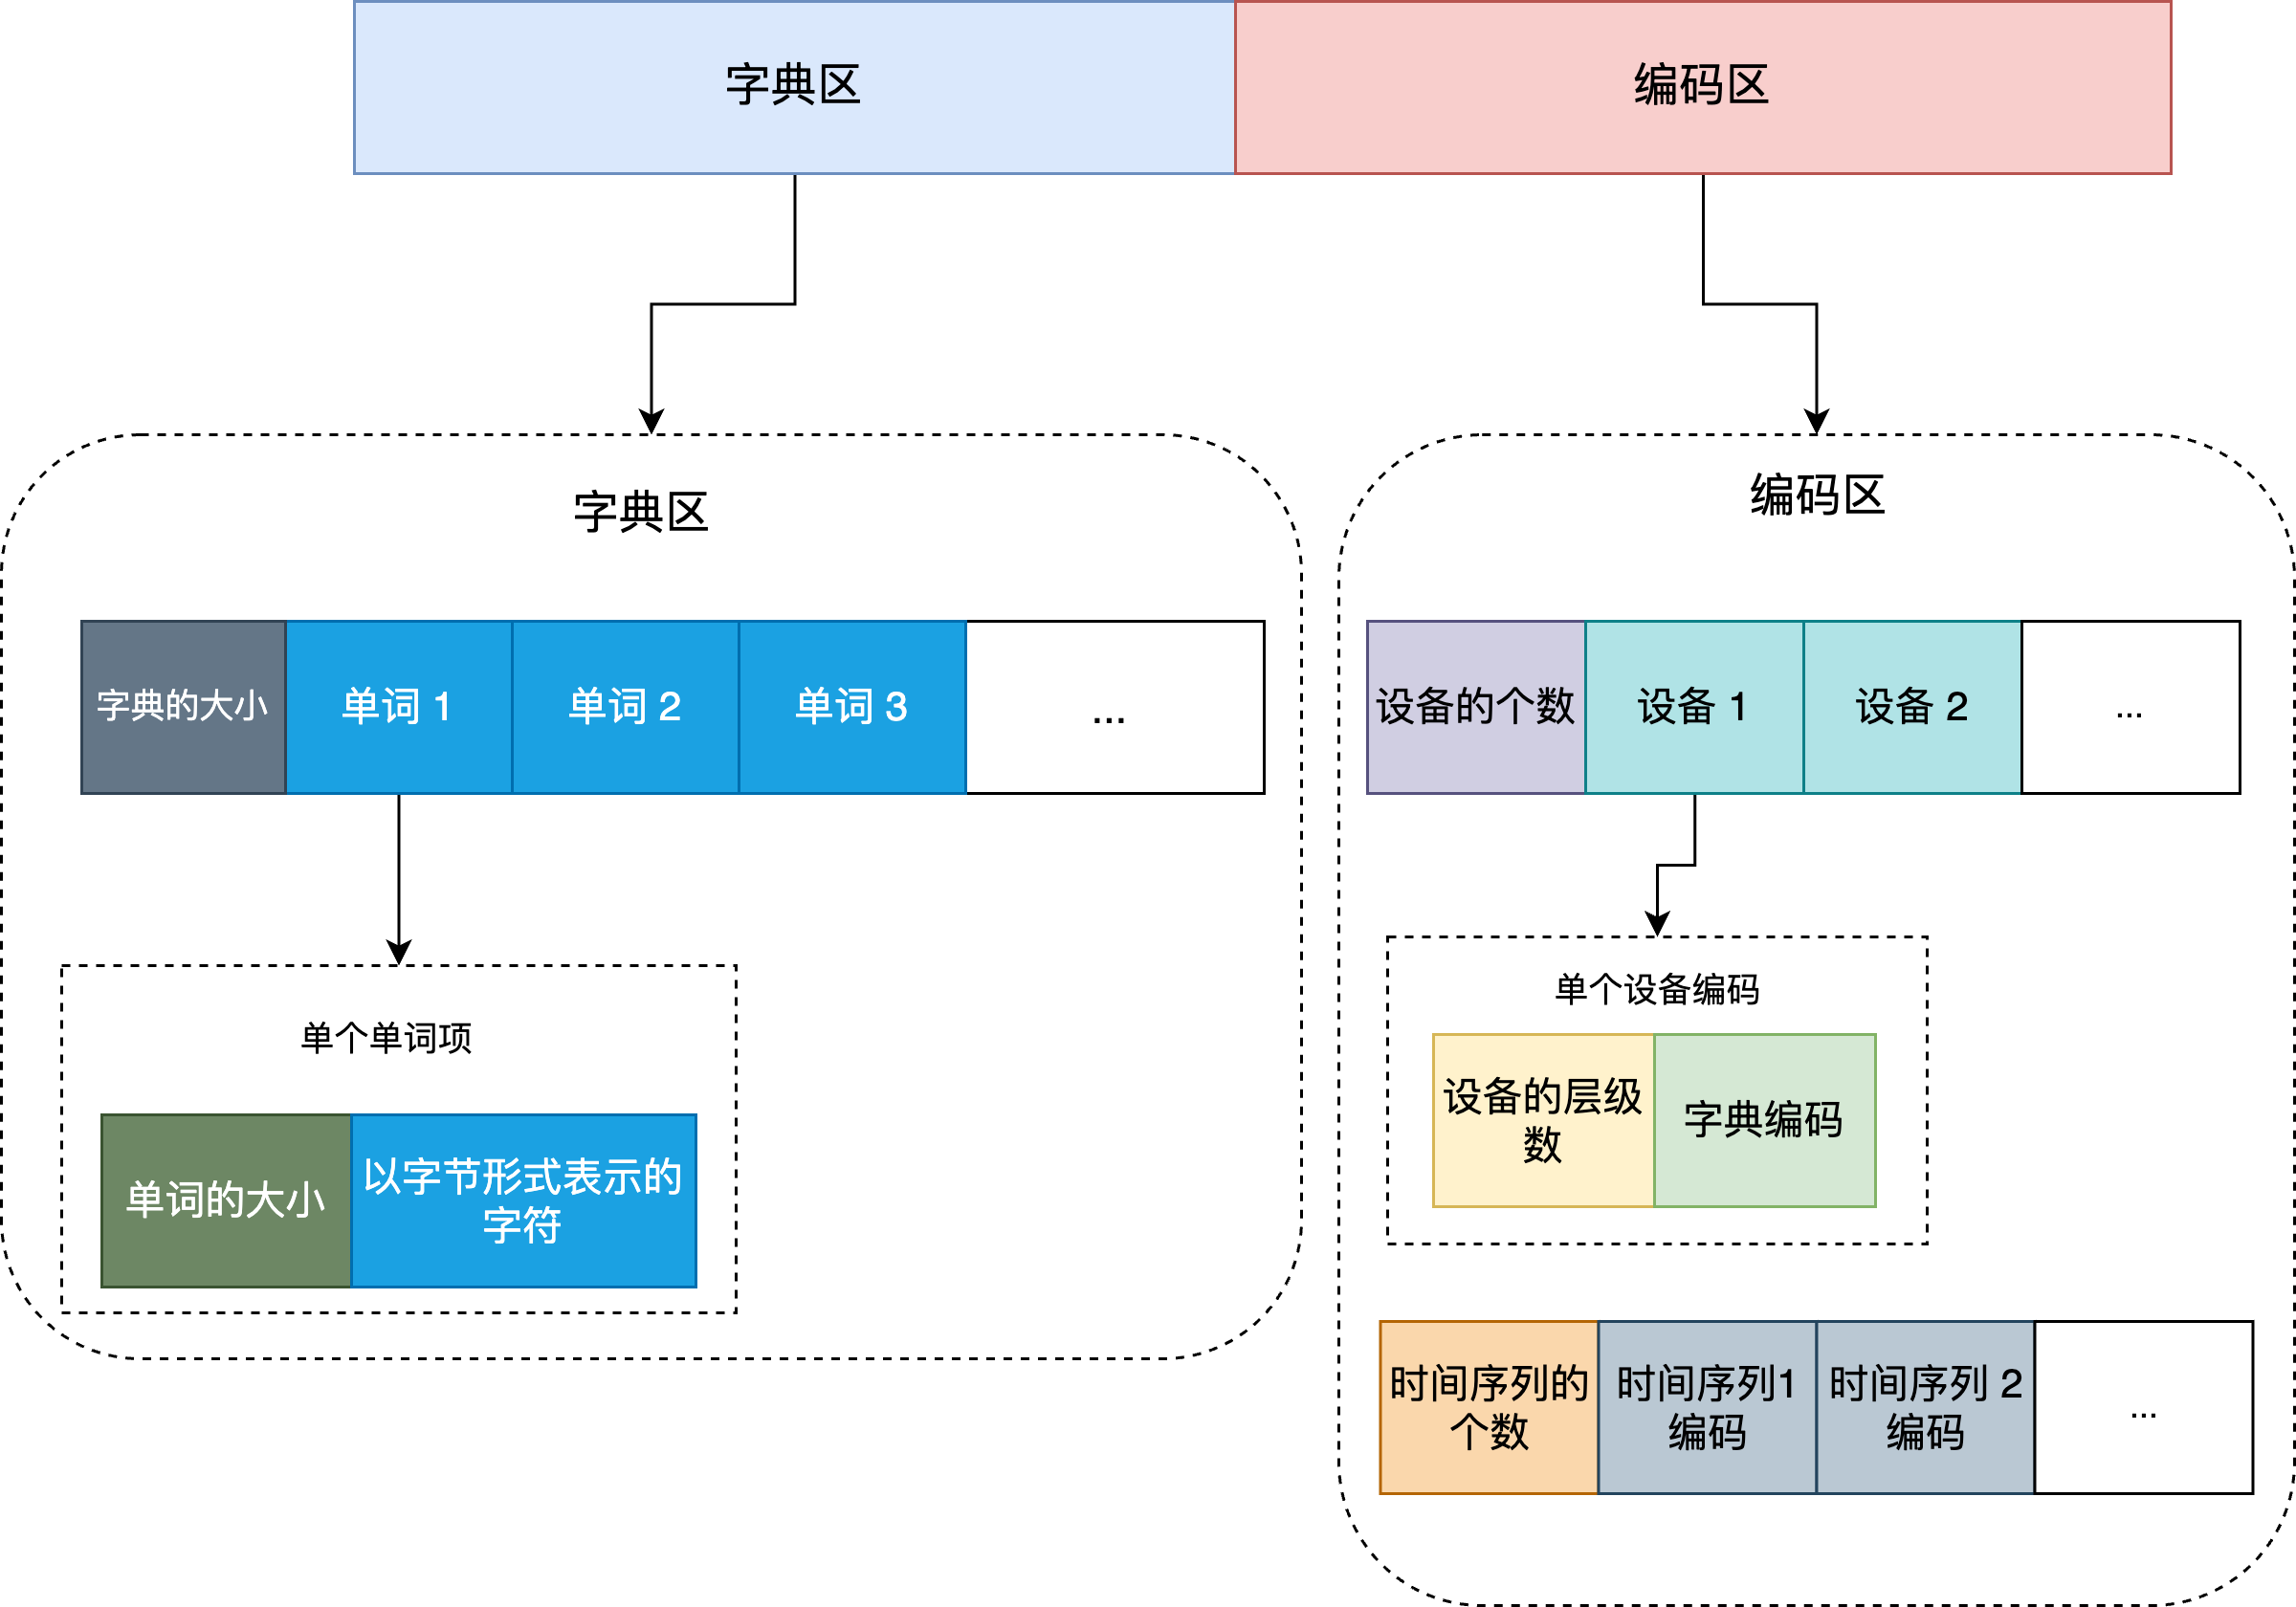
\includegraphics[width=\linewidth]{schema-encoding.png}
  \caption{元数据信息序列化方案设计}
  \label{fig:schema-encoding-general}
\end{figure}

图 \ref{fig:schema-encoding-general} 展示了对 \emph{insertRecords} 写入请求元数据信息序列化方案的总体设计。整体上,元数据信息采用了字典编码的方式进行序列化,字典编码的基本思想是利用一个字典来存储数据中重复出现的元素或模式,并用更短的编码来代替这些重复元素在原数据中的出现,以此来减少数据的体积。如果一个单词出现的频率越高,那么字典编码实现的数据压缩效果就越好。字典编码的核心步骤有两步:构建字典和利用字典进行编码。

 算法 \ref{alg:schema-build-dict} 展示了构建元数据信息序列化字典的过程。在 \emph{insertRecords} 的写入请求中,设备 ID 是一个带有层级结构的字符串,不同层级之间通过字符“.”分隔,形如 "root.层级1.层级2.层级3"。如果我们只是简单地将整个设备 ID 作为一个单词加入到字典中,那么只有当一个设备 ID 重复出现时,才有可能再次利用到这个单词。因为字典编码的压缩效果和单词的出现频率有关,所以为了提高单词的出现频率,本工作将一个设备按照层级拆分成多个单词,然后进行编码。例如 “root.sg.test.d1” 就会被拆分成 root、sg、test、d1 四部分,然后对每一个部分单独进行字典编码,并将编码后的结果拼凑到一起,例如如果 root 对应 1, sg 对应 5,test 对应 3,d1 对应 2,那么编码的结果就是 1532。在这样设计下,即使一个 \emph{insertRecords} 写入请求中的每一个设备 ID 都是不同的,只要这些设备之间存在一些共同的前缀,也都可以通过字典编码进行一定程度的压缩。

与设备 ID 不同,时间序列 ID 则是一个没有层级结构的字符串,不同设备之间可能存在时间序列 ID 相同的序列,因此直接使用整个时间序列 ID 进行编码也可以得到一定的压缩效果。为了更加充分地提高压缩效果,在本工作的设计中,设备 ID 和时间序列 ID 的编码使用共同的字典,因为越大的字典越能挖掘出潜在的编码可能性。

\begin{figure}
  \centering
  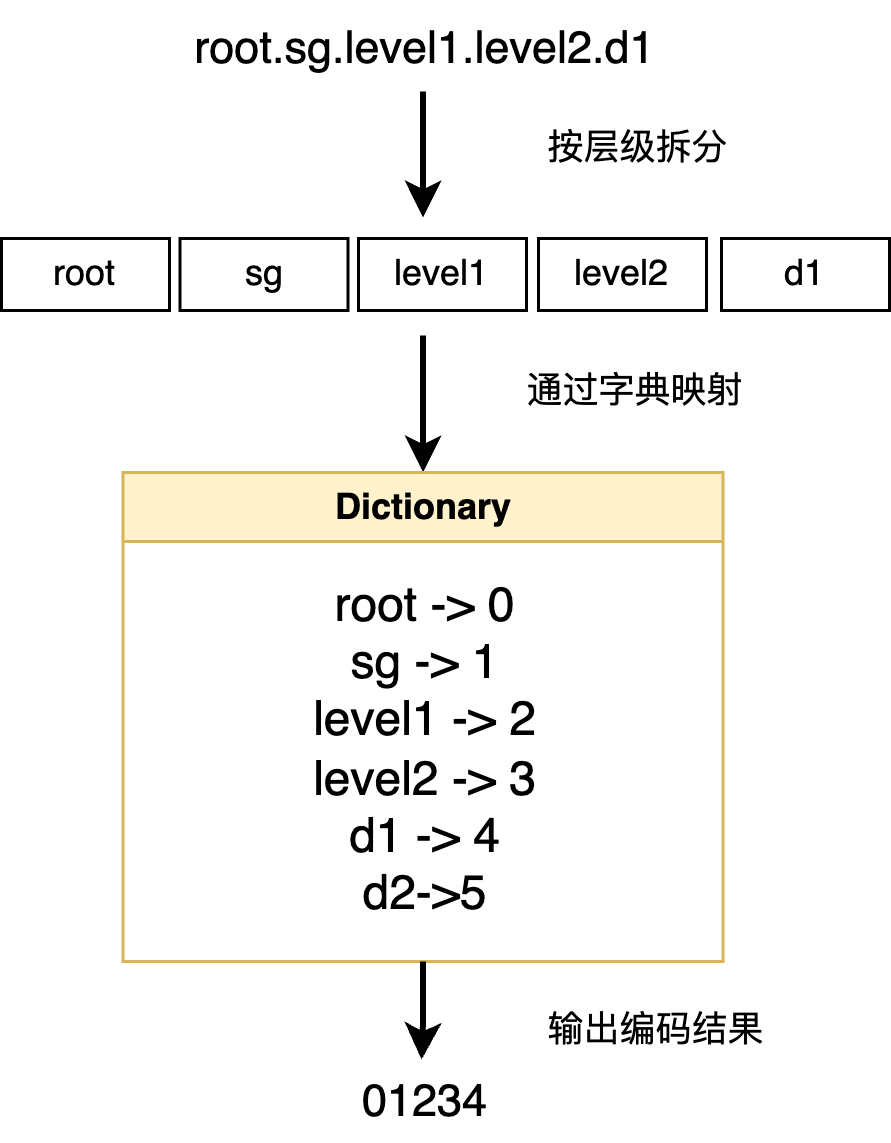
\includegraphics[width=0.55\linewidth]{device-id-encoding-process.png}
  \caption{每一个设备 ID 编码的过程}
  \label{fig:device-id-encoding}
\end{figure}

\begin{algorithm}
  \caption{元数据信息序列化过程构建字典流程}
  \label{alg:schema-build-dict}
  \small
  \begin{algorithmic}
    \REQUIRE \emph{deviceIds} 设备 ID 列表,\emph{timeseriesIDsList} 时间序列 ID 列表

    \STATE 创建一个保序哈希表 \emph{dict}
    \STATE $n\leftarrow$ \emph{deviceIds}.length
    \STATE \emph{counter} $\leftarrow 1$
    \FOR{$i=1$ to $n$}
      \STATE \emph{deviceId} = \emph{deviceIds}.at($i$)
      \STATE 将 \emph{deviceId} 按照 "." 进行切分,得到字符串数组 \emph{words}
      \FOR{\emph{word} in \emph{words}}
        \IF{\emph{word} 不在 \emph{dict} 中}
          \STATE 在 \emph{dict} 中构建映射 \emph{word} $\rightarrow$ \emph{counter}
          \STATE \emph{counter}$++$
        \ENDIF
      \ENDFOR
    \ENDFOR
    \STATE $n \leftarrow$ \emph{timeseriesIDsList}.length
    \FOR{$i=1$ to $n$}
      \STATE \emph{timeseriesIDs} $\leftarrow$ \emph{timeseriesIDsList}.at($i$)
      \STATE $m \leftarrow$ \emph{timeseriesIDs}.length
      \FOR{$j=1$ to $m$}
        \STATE $id \leftarrow$ \emph{timeseriesIDs}.at($j$)
        \IF{\emph{id} 不在 \emph{dict} 中}
          \STATE 在 \emph{dict} 中构建映射 \emph{id} $\rightarrow$ \emph{counter}
          \STATE \emph{counter}$++$
        \ENDIF
      \ENDFOR
    \ENDFOR

    \RETURN \emph{dict}

  \end{algorithmic}
\end{algorithm}

得到字典以后,就需要根据字典对元数据进行编码,主要分为对设备 ID 的编码和时间序列 ID 的编码。对设备的编码比较简单,因为设备 ID 列表是一个单层的列表,所以在编码之前先记录设备 ID 列表的长度。在对每个设备 ID 编码时,先将其按层级拆分,然后记录其层级数,再记录其每个层级所对应的编码值。在对时间序列 ID 进行编码时,因为它是一个两层嵌套的列表,因此不仅要记录外层的长度,也要记录内层每个列表的长度,然后进行查表序列化即可。

前面流程中所得到的字典也需要序列化为字节流,为了便于反序列化,我们将字典所对应的字节流放在了编码结果的前面。在将字典序列化为字节流时需要注意序列化的顺序,因为理论上我们需要记录每个单词所对应的编码值,但是我们为了节省这一部分开销,选择用单词在字典中的位置来代表它所对应的编码值。例如字典中出现的第一个单词就对应编码值 1,第二个单词对应 2,以此类推。算法 \ref{alg:schema-build-encoding} 描述了字典与编码的整个流程。

\begin{algorithm}
  \caption{元数据信息序列化构建编码结果的流程}
  \label{alg:schema-build-encoding}
  \small
  \begin{algorithmic}
    \REQUIRE \emph{deviceIds} 设备 ID 列表,\emph{timeseriesIDsList} 时间序列 ID 列表,\emph{dict} 编码字典

    \STATE 构建一个空字节流 \emph{buffer}
    \STATE 向 \emph{buffer} 中写入 \emph{dict} 的大小
    \FOR{字典中的每一个单词 \emph{word}}
      \STATE 向 \emph{buffer} 中写入 \emph{word} 的长度
      \STATE 向 \emph{buffer} 中写入 \emph{word} 的每一个字母
    \ENDFOR
    
    \STATE 向 \emph{buffer} 中写入 \emph{deviceIds} 的大小
    \FOR{\emph{deviceIds} 中的每一个 \emph{deviceId}}
      \STATE 将 \emph{deviceId} 按照 "." 切分成多个字符串,得到字符串数组 \emph{words}
      \STATE 向 \emph{buffer} 中写入 \emph{words} 的大小
      \FOR{\emph{words} 中的每一个 \emph{word}}
        \STATE 从 \emph{dict} 中查找 \emph{word} 所对应的编码 $e$
        \STATE 将 $e$ 写入到 \emph{buffer} 中
      \ENDFOR
    \ENDFOR

    \STATE 向 \emph{buffer} 中写入 \emph{timeseriesIDsList} 的大小
    \FOR{\emph{timeseriesIDsList} 中的每一个 \emph{timeseriesIDs}}
      \STATE 向 \emph{buffer} 中写入 \emph{timeseriesIDs} 的大小
      \FOR{\emph{timeseriesIDs} 中的每一个 \emph{timeseriesID}}
      \STATE 从 \emph{dict} 中查找 \emph{timeseriesID} 所对应的编码 $e$
      \STATE 向 \emph{buffer} 中写入 $e$
      \ENDFOR
    \ENDFOR

    \RETURN \emph{buffer}


  \end{algorithmic}
\end{algorithm}

\subsection{反序列化过程}
反序列化是序列化的逆过程,算法 \ref{alg:schema-decoding} 描述了元数据信息反序列化的过程。反序列化时先读取字典编码的字典,每个单词所对应的编码值由它在字典中出现的顺序所决定,算法一边读取单词,一边构建一个从编码值到单词的映射表。

将字典反序列化结束以后,就可以逐个读取设备 ID 的和时间序列 ID 的编码值,然后从编码值中恢复这些 ID。因为设备 ID 和时间序列 ID 分别以列表和嵌套列表的形式出现,因此解编码时也要根据字节流中所记录的列表长度信息对列表结构进行还原。


\begin{algorithm}
  \caption{元数据信息反序列化过程}
  \label{alg:schema-decoding}
  \small
  \begin{algorithmic}
    \REQUIRE \emph{buffer} 包含元数据信息的数据字节流
    \STATE 从 \emph{buffer} 中读取字典的大小 $n$
    \STATE 创建哈希表 \emph{dict}
    \FOR{$i=1$ to $n$}
      \STATE 从 \emph{buffer} 读取一个单词的长度 $m$
      \STATE 从 \emph{buffer} 中读取 $m$ 个字符,并构建成一个新的单词 \emph{word}
      \STATE 在 \emph{dict} 中添加映射: $i \rightarrow $ \emph{word}
    \ENDFOR

    \STATE 创建空列表 \emph{deviceIds}
    \STATE 从 \emph{buffer} 中读取设备 ID 的个数 $n$
    \FOR{$i=1$ to $n$}
      \STATE 从 \emph{buffer} 中读取当前设备的层级数 $k$
      \FOR{$j=1$ to $k$}
        \STATE 从 \emph{buffer} 中读取编码值 $e$
        \STATE 从 \emph{dict} 中根据 $e$ 查找到对应的单词
      \ENDFOR
      \STATE 将搜集到的单词拼装起来,使用 "." 连接,并加入到 \emph{deviceIds} 中
    \ENDFOR

    \STATE 创建空列表 \emph{timeseriesIdsList}
    \STATE 从 \emph{buffer} 中读取时间序列列表的个数 $n$
    \FOR{$i=1$ to $n$}
      \STATE 从 \emph{buffer} 中读取当前时间序列列表的长度 $m$
      \STATE 创建一个空列表 \emph{timeseriesIds}
      \FOR{$j=1$ to $m$}
        \STATE 从 \emph{buffer} 中读取编码值 $e$
        \STATE 从 \emph{dict} 中读取对应的单词,并添加到 \emph{timeseriesIds} 中
      \ENDFOR
      \STATE 将 \emph{timeseriesIds} 添加到 \emph{timeseriesIdsList} 中
    \ENDFOR

    \RETURN \emph{deviceIds}, \emph{timeseriesIdsList}

  \end{algorithmic}
\end{algorithm}


\section{数据部分序列化与反序列化方案设计}
\subsection{序列化过程}
对写入请求进行序列化的过程其实本质上是将一份数据转换成字节流,然后传递给下一个处理流程。这个本质与数据存储是类似的,只不过前者将数据交由网络进行传输,而数据存储则将序列化得到的字节流交由磁盘进行存储。因此,我们可以借鉴数据存储领域的一些设计思想。

目前数据库数据存储主要有三种方案:行式存储(Row Storage)、列式存储(Columnar Store)和混合存储(Hybrid Store)。行式存储将一行数据一起保存,相邻的数据项来自不同的列,它们可能类型不同,或者类型相同但是数值的分布不同;列式存储则是将一列数据保存在一起,相邻的数据项不仅类型相同,它们的数值也遵循着共同的分布;混合存储则是将行式存储和列式存储的设计相结合,先将数据按行进行分割成多个块,然后在每个块中按照列的形式存储。行式存储的优势是同一行的数据被聚集在一起,可以方便地访问同一行中的多项数据;列式存储的优势是可以获得更好的压缩比,减少数据体积;混合存储则在一定程度上结合了两者的优势。

同样的,在对写入请求进行序列化时,也可以选择行式存储、列式存储和混合存储。行式存储就是将每一条 Record 的数据一起序列化,列式存储将一条时间序列的数据单独序列化,而混合存储则是先将 Records 分成多批,在每一批内进行列式序列化。

行式序列化的优点在于实现简单,这是因为序列化时一条数据的多个数据项只需要按照顺序逐个转换为字节并添加到字节流中即可,反序列化时也可以按照顺序读取字节流并逐个反序列化单个数据项。但是行式序列化将不同类型的数据全部混合到了一起,导致在压缩时没有办法根据数据的特点进行优化,只能使用通用的压缩算法(如 Snappy\cite{samulowitz2013snappy}、GZip\cite{deutsch1996gzip}、ZSTD\cite{collet2018zstandard} 等)对整体进行压缩,无法实现更加精细化、高效的压缩。

普通的列式序列化将一条时间序列的全部数据都放到一起进行编码,这样数据不仅类型相同,而且都遵循类似的分布,压缩的效果更好。但是,在一个 \emph{insertRecords} 写入请求中,同一条时间序列的数据不会太多,如果只把一条时间序列的若干个数据点放到一起压缩,效果也不好。

为了获取较好的压缩效果,本工作改进了普通列式序列化方案,设计了一种以数据类型为聚集单位的列式序列化方案。图 \ref{fig:value-encoding-general} 展示了数据部分序列化的整体设计,序列化的结果一共分为 3 个区域:时间戳区、数据区和数据类型区。其中,时间戳区只包含时间戳,其中的内容是一个 \emph{insertRecords} 请求中所有记录的时间戳,每个时间戳的大小都固定为 8 字节。数据区包含了具体的数值项,并且这些数值项根据它们的类型被聚集在一起,同一条记录或者不同记录中有相同类型的数据会位于相邻的位置,而同一条记录中类型不同的数据则可能位于较远的位置。除文本类型外,同一数据类型内每个数据项的长度都是相同的。最后一个区域是数据类型区,其包含了写入请求中每个数据项的类型,以及每一行记录的长度。

这样设计的好处在于,我们可以根据每个区域的特点为它们选择合适的压缩算法,而不是只能使用通用的压缩算法进行粗暴的压缩。例如,对于时间戳区,在同一个写入请求中的时间戳通常在数值上都非常接近,因此我们可以选择 Gorilla\cite{pelkonen2015gorilla} 压缩算法对其进行压缩,因为 Gorilla 算法尤其适合用于那些数值波动范围较小的数据;对于 Bool 类型,由于只有 True 和 False 两种取值,我们可以将原本用一个字节表示的数据项变成 1 个 bit,节省了 8 倍的空间。

\begin{figure}
  \centering
  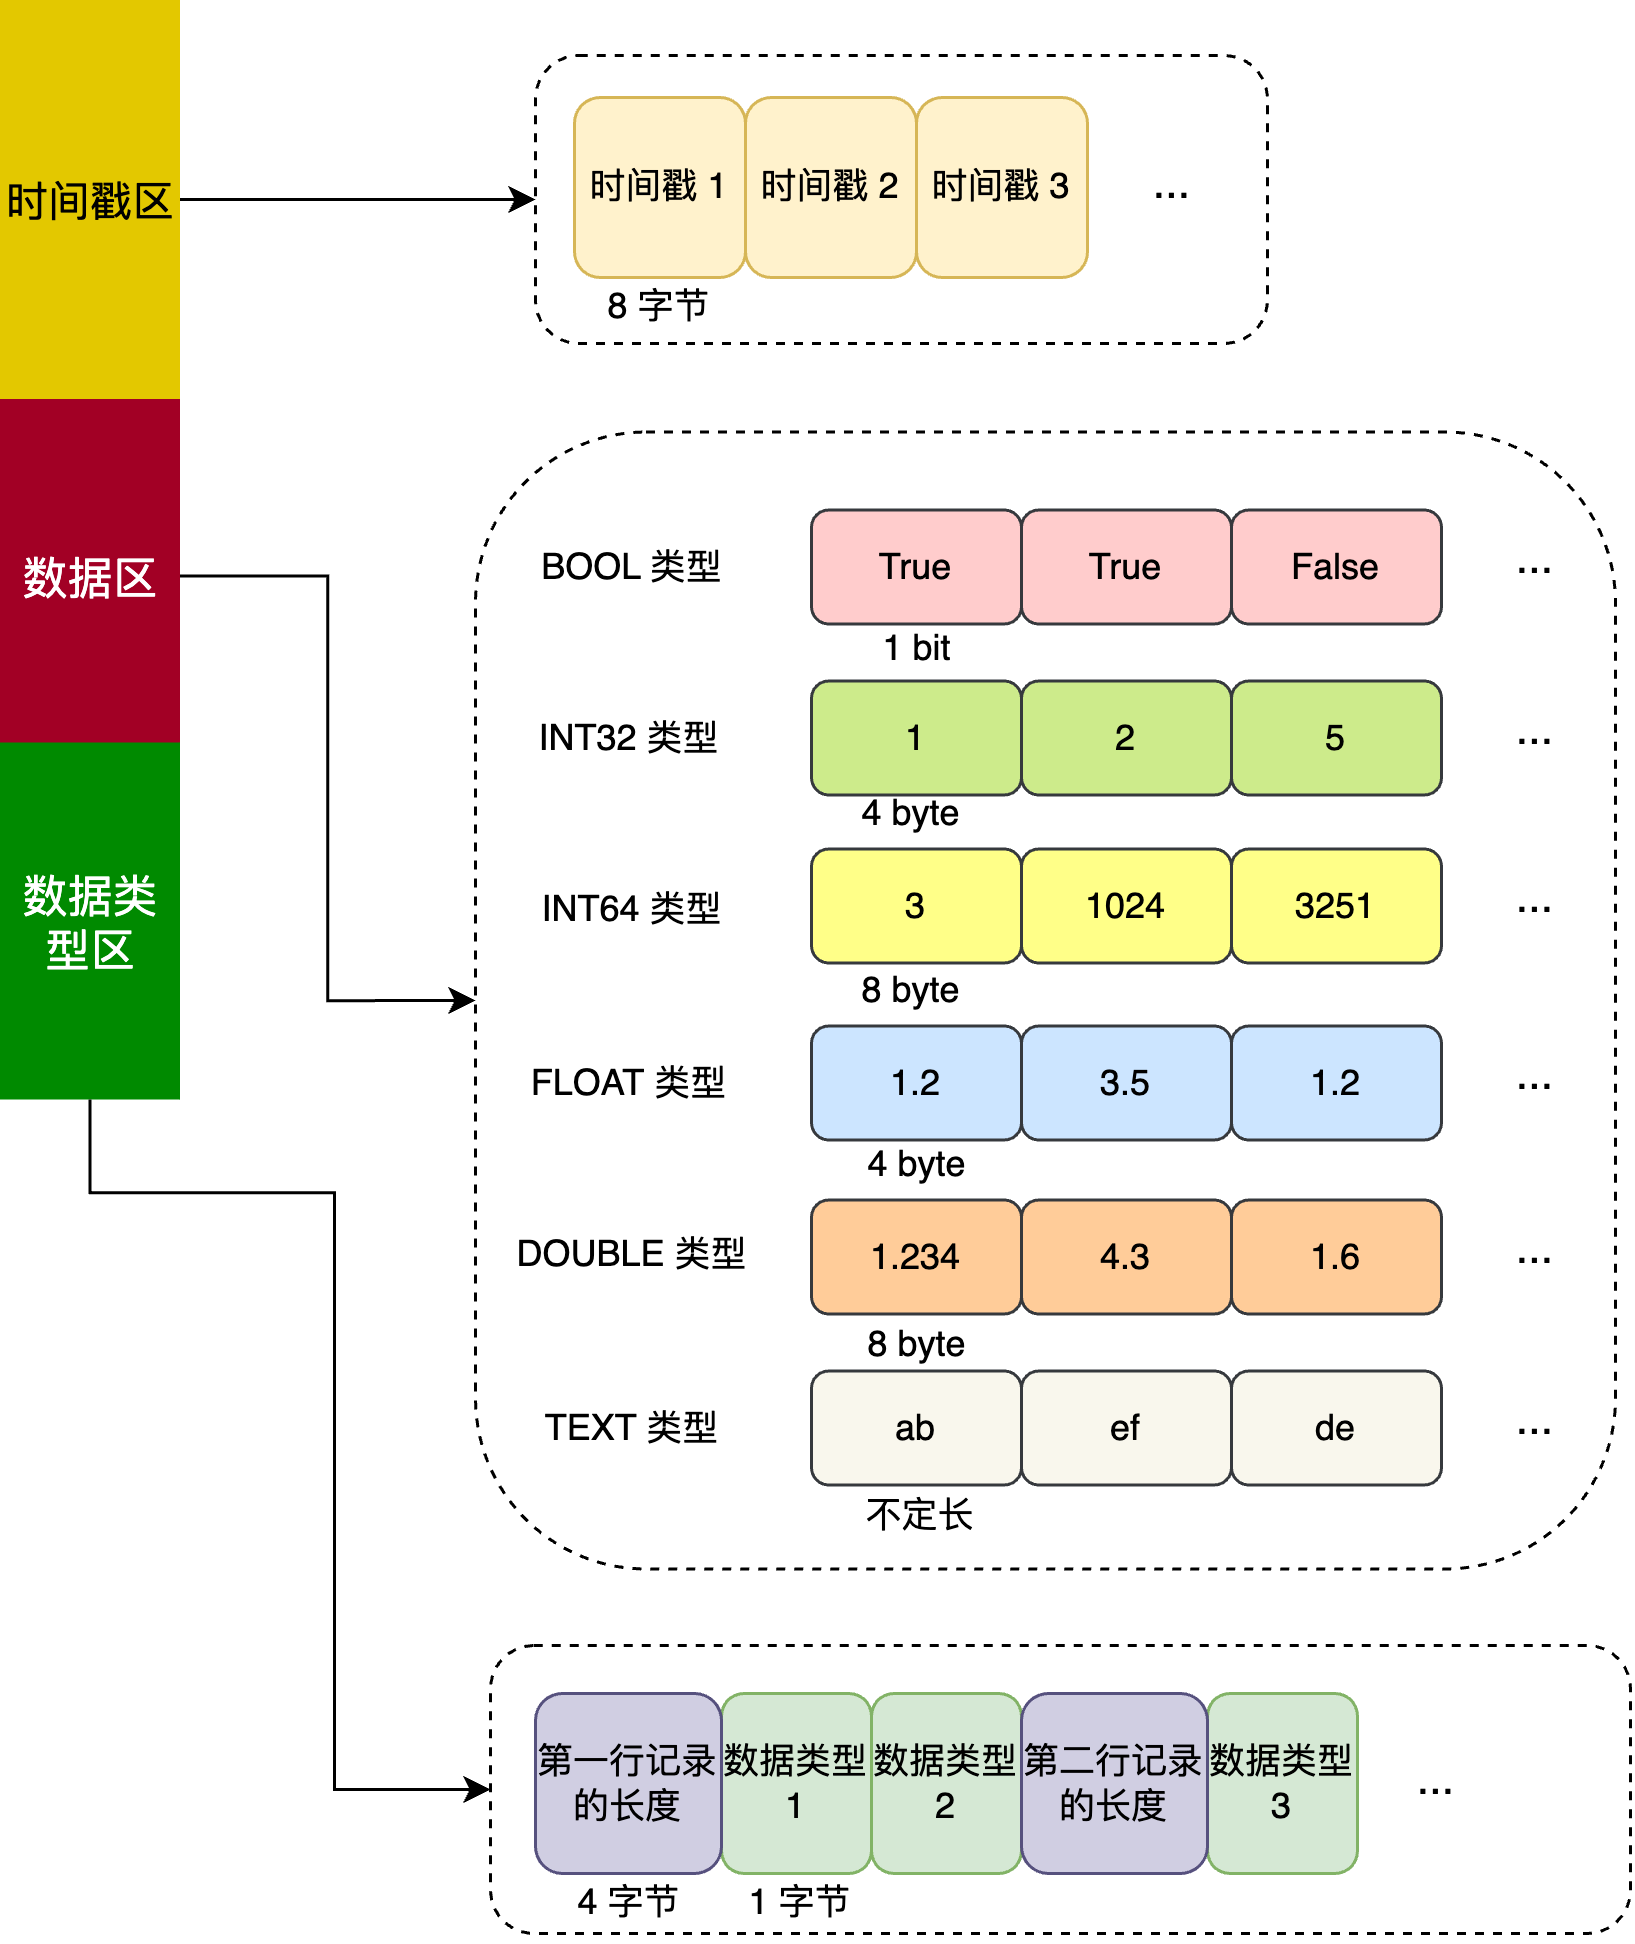
\includegraphics[width= 0.9\linewidth]{value-encoding.png}
  \caption{数据部分序列化设计}
  \label{fig:value-encoding-general}
\end{figure}

算法 \ref{alg:value-encoding} 描述了对写入请求数据部分进行序列化的过程。首先是处理时间戳的部分,将时间戳逐一序列化到一个字节流中,然后使用 Gorilla 压缩算法压缩这个字节流。然后是处理数据的部分,首先将数据按照类型分类,放到多个不同类型的数据列表中,然后将这些数据列表分别进行压缩,最后将压缩后的结果序列化到一个字节流中。在压缩时,我们可以根据数据类型的不同选择合适的压缩算法,如对数值类型选择 Gorilla 算法,这是一种无损的、适用于数据变化幅度不大的压缩算法;对文本类型使用字典压缩算法;对布尔类型使用 Bitpacking 压缩算法\cite{hwang2023lossless}。最后是处理数据类型的部分,将每一行记录的长度和每个数据项的类型序列化到一个字节流中,并最后将这个字节流写入到输出字节流中,数据部分的序列化就完成了。

\begin{algorithm}
  \caption{数据部分序列化过程}
  \label{alg:value-encoding}
  \small
  \begin{algorithmic}
    \REQUIRE \emph{timestamps} 时间戳列表,\emph{datatypesList} 数据类型列表,\emph{valuesList} 数据列表 
    \STATE 创建一个空的字节流 \emph{outputBuffer} 和一个空的字节流 \emph{timeBuffer}
    \STATE 向 \emph{outputBuffer} 中写入 \emph{timestamps} 的大小
    \FOR{\emph{timestamps} 中的每一个 \emph{timestamp}}
      \STATE 将 \emph{timestamp} 写入到 \emph{timeBuffer} 中
    \ENDFOR
    \STATE 对 \emph{timeBuffer} 使用 Gorilla 算法压缩,并将压缩后的结果写入到 \emph{outputBuffer} 中 

    \STATE 创建六个数据列表,分别对应不同的数据类型:\emph{boolList}、\emph{intList}、\emph{longList}、\emph{floatList}、\emph{doubleList}、\emph{textList}
    \STATE 创建一个空的字节流 \emph{typeBuffer}
    \STATE 创建变量 $n = $\emph{datatypesList}.length
    \STATE 将 $n$ 序列化到 \emph{typeBuffer} 中
    \FOR{$i=1$ to $n$}
      \STATE \emph{datatypes} $=$ \emph{datatypesList}.at($i$)
      \STATE 创建变量 $m = $\emph{datatypes}.length
      \STATE 将 $m$ 序列化到 \emph{typeBuffer} 中
      \FOR{$j=1$ to $m$}
        \STATE 根据 \emph{datatypes}.at($j$) 的类型,将 \emph{valuesList}.at($i$).at($j$) 放到对应的数据列表中
        \STATE 将 \emph{datatypes}.at($j$) 的值序列化到 \emph{typeBuffer} 中
      \ENDFOR
    \ENDFOR
    \STATE 将 \emph{boolList} 的大小序列化到 \emph{outputBuffer} 中
    \STATE 将 \emph{boolList} 中的数据按位表示序列化到 \emph{outputBuffer} 中
    \STATE 将 \emph{intList} 的大小序列化到 \emph{outputBuffer} 中
    \STATE 将 \emph{intList} 中的数据使用 Gorilla 压缩后序列化到 \emph{outputBuffer} 中
    \STATE 将 \emph{longList} 的大小序列化到 \emph{outputBuffer} 中
    \STATE 将 \emph{longList} 中的数据使用 Gorilla 压缩后序列化到 \emph{outputBuffer} 中
    \STATE 将 \emph{floatList} 的大小序列化到 \emph{outputBuffer} 中
    \STATE 将 \emph{floatList} 中的数据使用 Gorilla 压缩后序列化到 \emph{outputBuffer} 中
    \STATE 将 \emph{doubleList} 的大小序列化到 \emph{outputBuffer} 中
    \STATE 将 \emph{doubleList} 中的数据使用 Gorilla 压缩后序列化到 \emph{outputBuffer} 中
    \STATE 将 \emph{textList} 的大小序列化到 \emph{outputBuffer} 中
    \STATE 将 \emph{textList} 中的数据使用字典编码后序列化到 \emph{outputBuffer} 中
    \STATE 将 \emph{typeBuffer} 写入到 \emph{outputBuffer} 中
    \RETURN \emph{outputBuffer}

  \end{algorithmic}
\end{algorithm}
\subsection{反序列化过程}
\begin{algorithm}
  \caption{数据部分反序列化过程}
  \label{alg:value-decoding}
  \small
  \begin{algorithmic}
    \REQUIRE \emph{buffer} 包含数据部分的字节流
    \STATE 从 \emph{buffer} 中读取时间戳的个数 $n$
    \STATE 创建一个空的时间戳列表 \emph{timestamps}
    \STATE 创建 Gorilla 解压缩器 \emph{decompressor}
    \FOR{$i=1$ to $n$}
      \STATE 使用 \emph{decompressor} 从 \emph{buffer} 中读取一个时间戳 $t$
      \STATE 将 $t$ 添加到 \emph{timestamps} 中
    \ENDFOR
    \STATE 从 \emph{buffer} 中反序列化出布尔类型的数据列表 \emph{boolList}
    \STATE 从 \emph{buffer} 中反序列化出整数类型的数据列表 \emph{intList}
    \STATE 从 \emph{buffer} 中反序列化出长整数类型的数据列表 \emph{longList}
    \STATE 从 \emph{buffer} 中反序列化出浮点数类型的数据列表 \emph{floatList}
    \STATE 从 \emph{buffer} 中反序列化出双精度浮点数类型的数据列表 \emph{doubleList}
    \STATE 从 \emph{buffer} 中反序列化出文本类型的数据列表 \emph{textList}
    \STATE 从 \emph{buffer} 中读取数据类型列表的个数 $n$
    \STATE 创建一个空的数据类型列表 \emph{datatypesList},一个空的数据列表 \emph{valuesList}
    \FOR{$i=1$ to $n$}
      \STATE 从 \emph{buffer} 中读取当前数据类型列表的长度 $m$
      \STATE 创建一个空的数据类型列表 \emph{datatypes}
      \STATE 创建一个空的数据列表 \emph{values}
      \FOR{$j=1$ to $m$}
        \STATE 从 \emph{buffer} 中读取数据类型 $t$
        \STATE 将 $t$ 添加到 \emph{datatypes} 中
        \STATE 根据 $t$ 从对应的数据列表中读取数据 $v$,并从该数据列表中移除掉该元素
        \STATE 将 $v$ 添加到 \emph{values} 中
    \ENDFOR
    \ENDFOR
    \RETURN \emph{timestamps}, \emph{datatypesList}, \emph{valuesList}
  \end{algorithmic}
\end{algorithm}

算法 \ref{alg:value-decoding} 描述了数据部分反序列化的过程。反序列化时,首先读取时间戳的个数,然后逐一读取时间戳并添加到时间戳列表中。然后从字节流中读取布尔类型、整数类型、长整数类型、浮点数类型、双精度浮点数类型和文本类型的数据列表,并根据对应的压缩算法类型对它们进行解压缩,这些数据列表中的数据是按照序列化时的顺序排列的。最后读取数据类型列表的个数,然后逐一读取每个数据类型列表的长度,再逐一读取每个数据类型列表中的数据类型,每读取一个数据类型,就根据这个数据类型去对应的数据列表中读取最顶部的数据,然后将这个列表顶部的数据移除,并将这个数据添加到一个新的数据列表中。最后返回时间戳列表、数据类型列表和数据列表,反序列化过程就完成了。

\section{写入请求辅助信息部分序列化与反序列化方案设计}
\subsection{序列化流程}
\begin{figure}
  \centering
  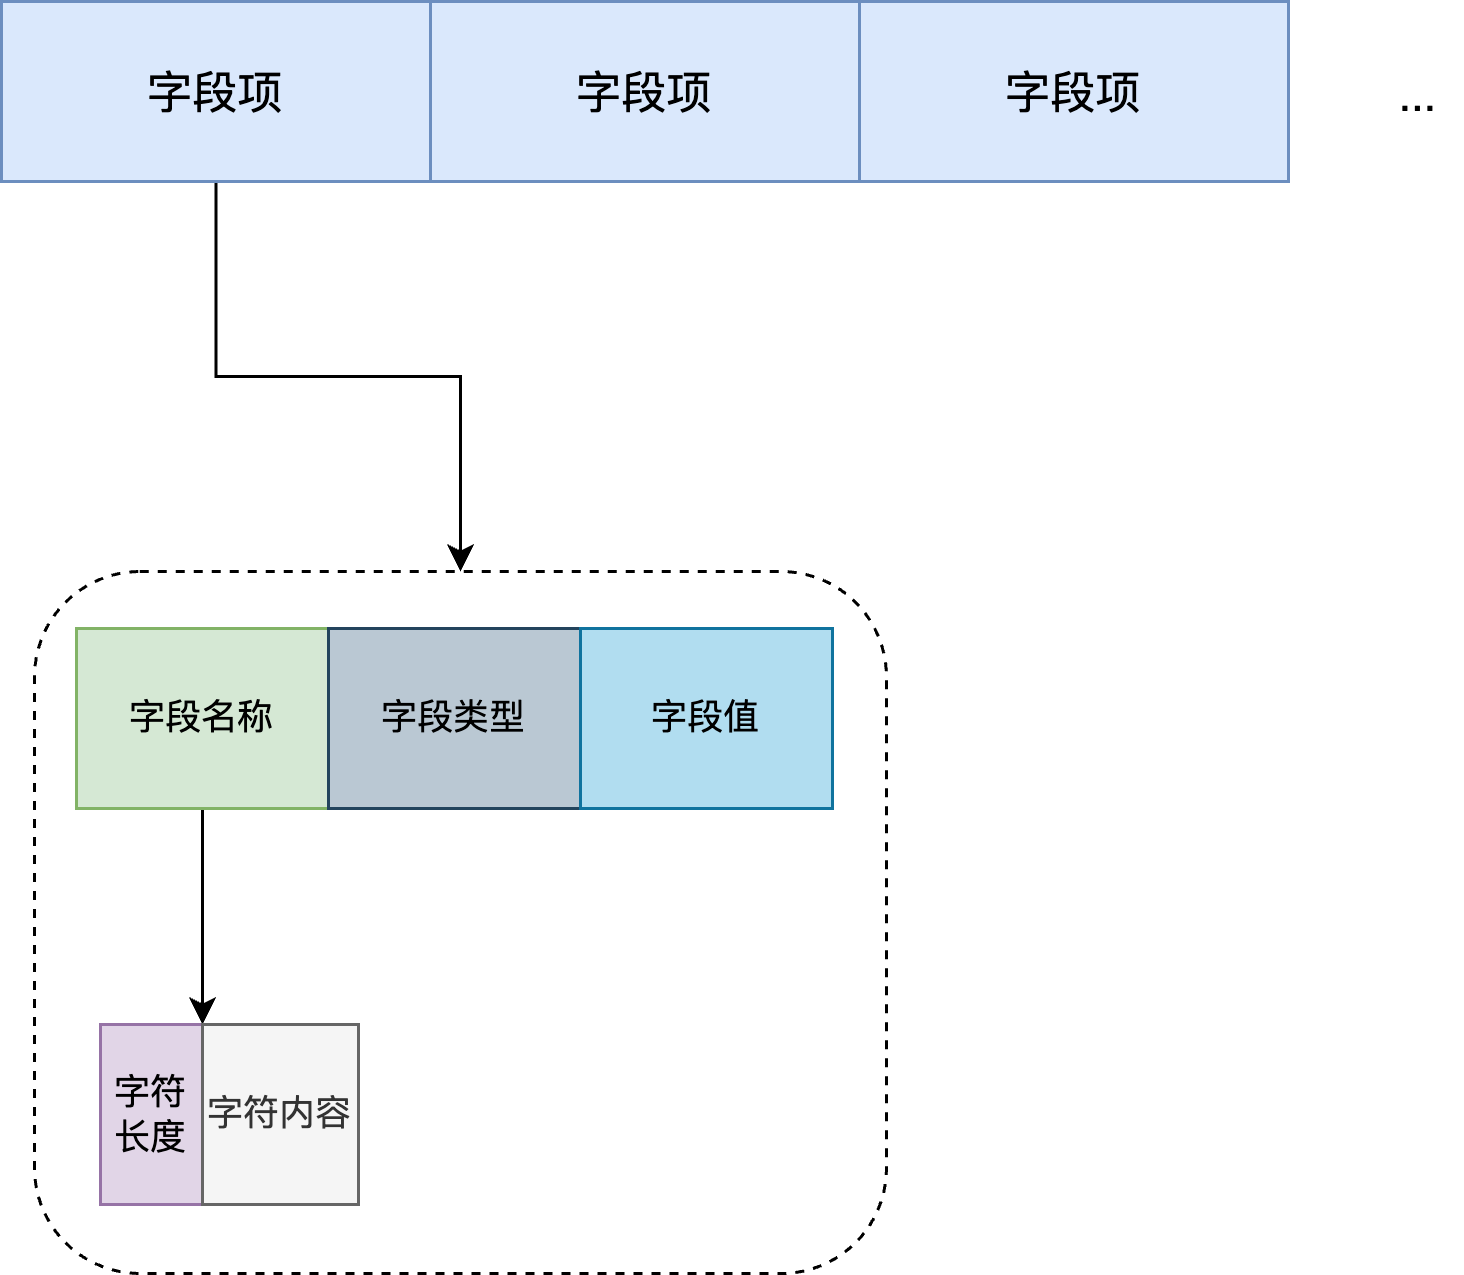
\includegraphics[width=0.75\linewidth]{auxiliary-buffer-design.png}
  \caption{辅助信息部分序列化设计}
  \label{fig:aux-encoding-general}
\end{figure}

辅助信息主要包含一些零散的字段,这些字段的数据类型可能不同,因此在序列化时需要对每个字段进行单独的处理。图 \ref{fig:aux-encoding-general} 展示了辅助信息部分序列化的整体设计。辅助信息部分序列化的结果分为一个个单独的字段项,每个字段项中包含了该字段的名称、该字段的类型以及该字段的值。

\begin{algorithm}
  \caption{辅助信息序列化过程}
  \label{alg:aux-encoding}
  \small
  \begin{algorithmic}
    \REQUIRE \emph{auxiliaryInfo} 辅助信息哈希表,表示从字段名到字段值的映射
    \STATE 创建一个空的字节流 \emph{outputBuffer}
    \STATE 创建变量 $n = $\emph{auxiliaryInfo}.size
    \STATE 将 $n$ 序列化到 \emph{outputBuffer} 中
    \FOR{哈希表中的每一个键值对 (\emph{name}, \emph{value})}
      \STATE 将 \emph{name} 序列化到 \emph{outputBuffer} 中
      \STATE 将 \emph{value} 的类型序列化到 \emph{outputBuffer} 中
      \STATE 根据 \emph{value} 的类型将 \emph{value} 序列化到 \emph{outputBuffer} 中
    \ENDFOR
    \RETURN \emph{outputBuffer}
  \end{algorithmic}
\end{algorithm}

算法 \ref{alg:aux-encoding} 展示了辅助信息序列化的过程。算法的输入是一个哈希表,其中包含了从辅助字段名到字段内容的映射。首先,程序将该哈希表的大小序列化到字节流中,然后遍历哈希表中的每一个键值对,将键值对的键(字段名)、字段类型以及值(字段内容)分别序列化到字节流中,最后输出序列化得到的字节流。

\subsection{反序列化流程}
\begin{algorithm}
  \caption{辅助信息反序列化过程}
  \label{alg:aux-decoding}
  \small
  \begin{algorithmic}
    \REQUIRE \emph{buffer} 包含辅助信息的字节流
    \STATE 从 \emph{buffer} 中读取哈希表的大小 $n$
    \STATE 创建一个空的哈希表 \emph{auxiliaryInfo}
    \FOR{$i=1$ to $n$}
      \STATE 从 \emph{buffer} 中读取字段名 \emph{name}
      \STATE 从 \emph{buffer} 中读取字段类型 \emph{type}
      \STATE 根据 \emph{type} 从 \emph{buffer} 中读取字段值 \emph{value}
      \STATE 将 (\emph{name}, \emph{value}) 添加到 \emph{auxiliaryInfo} 中
    \ENDFOR
    \RETURN \emph{auxiliaryInfo}
  \end{algorithmic}
\end{algorithm}

算法 \ref{alg:aux-decoding} 展示了辅助信息反序列化的过程。算法的输入是一个字节流,其中包含了序列化得到的辅助信息。首先,程序从字节流中读取哈希表的大小,然后创建一个空的哈希表。接着,程序遍历字节流中的每一个字段项,从中读取字段名、字段类型和字段值,并将这些信息添加到哈希表中。最后,程序返回反序列化得到的哈希表。上层程序可以使用字段名从该哈希表中检索该字段所对应的数据。如果需要增加新的辅助字段,那么只需要在哈希表中添加新的键值对即可,具有良好的扩展性,满足了设计需求。

\section{新 \emph{insertRecords} 写入请求序列化与反序列化实现}
本工作对上述的设计进行了实现,因为 IoTDB 使用 Apache Thrift 进行远程服务调用,因此本工作的实现也仍然没有脱离 Thrift 的框架,但将字段与内容的序列化和反序列化过程自行实现,序列化后的内容通过 Thrift 进行传输。新的 \emph{insertRecords} 写入接口在 Thrift IDL 中定义如下:
\begin{lstlisting}[language=idl,frame = trBL , escapeinside={(*@}{@*)}]
struct TSInsertRecordsReq {
  1: required binary schemaBuffer,
  2: required binary valueBuffer,
  3: required binary auxiliaryBuffer
}
  
TSStatus insertRecords(1:TSInsertRecordsReq req);
\end{lstlisting}
TSInsertRecordsReq 结构体中的 schemaBuffer、valueBuffer、auxiliaryBuffer 分别对应了元数据信息、数据部分和辅助信息的序列化结果,这三个字节流数据的序列化和反序列化过程由我们自行实现。

除了前文中描述的序列化与反序列化算法,为了减小数据包的体积,我们还对由上述算法产生的字节流分别进行了压缩。压缩被实现为可选的,在字节流中通过一个标志位来表示是否进行了压缩,图 \ref{fig:compress-rpc-buffers} 展示了经过加上压缩之后 RPC 字节流的结构。当字节流被压缩过,最前面的标志位会被置为 1,并且原始数据包的长度也被记录在字节流中;如果字节流没有被压缩过,那么标志位为 0,并且紧随其后的就是原始的字节流如果字节流被压缩过,那么在反序列化之前需要先对数据进行解压缩;反之,程序可以直接对字节流进行反序列化。

\begin{figure}
  \centering
  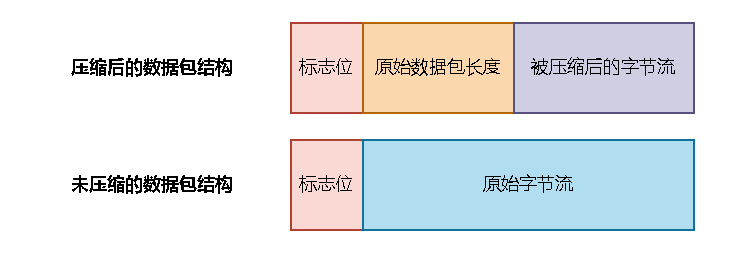
\includegraphics[width=\linewidth]{compress-rpc-buffers.pdf}
  \caption{压缩后的 RPC 字节流结构}
  \label{fig:compress-rpc-buffers}
\end{figure}

最后,在实现时,结合 Java 语言的特性,为了提高序列化和反序列化的性能,我们使用了 DirectByteBuffer 来进行字节流的读写操作,这样可以避免数据在内存中的拷贝,也可以减轻系统垃圾回收的频率,提高了序列化和反序列化的效率。

\section{本章小结}
本章首先介绍了 \emph{insertRecords} 写入请求序列化的设计目标,然后分别介绍了对写入请求中元数据部分、数据部分以及辅助信息部分的序列化与反序列设计。元数据部分的序列化利用了设备 ID 与时间序列 ID 都是重复性高的文本的特点,利用字典编码减少序列化后数据的体积;数据部分的序列化使用了以数据类型为聚集单位的列式存储设计,根据数据类型的不同选择合适的压缩算法,提高了压缩效果;辅助信息部分的序列化则是将每个字段的名称、类型和值分别序列化到字节流中,具有良好的扩展性。最后,本章介绍了在对写入请求序列化与反序列化实现时的一些细节。